\subsection{Matrix element for the $Z^+ \to \psi K^+$ chain}
The chain of $\Bp\to \Z^+_j \phi$, $Z^+_j\to \psi K^+$, $\phi\to K^+K^-$,  $\psi\to \mu^+\mu^-$ also contains four terms. 
The $\Bs\to \Z^+_j \phi$ gives a term, $\H^{B\to Z_j \phi}_{\lambda_{\phi}^Z}$ and limits $\lambda_{Z}=\lambda_{\phi}^Z$. 
The superscript $Z$ in $\lambda_{\phi}$ accounts for different helicity frame than that in the $K^*$ chain. 

The $Z^+_j \to \psi K^+$ is described by one term 
\begin{equation}
\H_{\lambda_\psi^{Z}}^{Z_{j}}D^{\,\,J_{Z_j}}_{\lambda_Z,\,\lambda_\psi^{Z}}(\phi_\psi^Z,\theta_{Z},0)^*R_{Z_j}(m_{\psi K}),
\end{equation}
The helicity angles of $Z$ decays $\phi_\psi^Z$ and $\theta_{Z}$ are defined by the $\psi$ direction. 
The strong decay conserve parity, which gives the relation $\H_{-\lambda_\psi^{Z}}^{Z_{j}}=(-1)^{J_{Z_j}-1}P_{Z_j}\H_{\lambda_\psi^{Z}}^{Z_{j}}$.

The $\phi\to K^+K^-$ provides one term 
\begin{equation}
D^{\,\,1}_{\lambda^Z_{\phi},\,0}(\phi^Z_{K^+},\theta^Z_\phi,0)^*,
\end{equation}
where $K^+$ is used to define the two helicity angles of $\phi^Z_{K^+}$ and $\theta^Z_\phi$ from $\phi$ decays. We use the superscript $Z$ to differentiate from the $\Kst$ chain. 

The $\psi\to\mu^+\mu^-$ decay is described by the term
\begin{equation}
D^{\,\,1}_{\lambda^{Z}_{\psi},\,\Delta\lambda^{Z}_\mu}(
\phi_{\mu}^{Z},\theta_{\psi}^{Z},0)^*.
\end{equation}
Since the muons are final-state particles,
their helicity states in the $Z$ decay chain, $|\lambda_\mu^{Z}\rangle$, 
need to be rotated to the muon helicity states in the $f$ decay chain, $|\lambda_\mu\rangle$, 
before the $Z$ matrix element terms can be coherently added to the $f$ matrix element terms. 
The term aligning the muon helicity states between the two reference frames is given by
\begin{equation}
   \sum\limits_{\lambda_\mu^{Z}} D^{\,\,J_\mu}_{\lambda_\mu^{Z}\,\lambda_\mu}(\alpha^{Z}_\mu,0,0)^* =
 \sum\limits_{\lambda_\mu^{Z}} e^{i\,\lambda_\mu^{Z}\alpha^{Z}_\mu} \delta_{\lambda_\mu^{Z},\,\lambda_\mu}
= e^{i\,\lambda_\mu\alpha^{Z}_\mu}.
\end{equation}
The transformation of $\mu^-$ states will be similar to that of the $\mu^+$ states, except that since $\hat{z}_\psi$ will have the opposite direction, 
$\alpha^{Z}_{{\mu^+}} = - \alpha^{Z}_{\mu^-}$. 
The transformation of $|\lambda_{\mu^+}^{Z}\rangle|\lambda_{\mu^-}^{Z}\rangle$ 
to $|\lambda_{\mu^+}\rangle|\lambda_{\mu^-}\rangle$ states will require multiplying the terms for the $Z$ decay chain by 
\begin{equation}
  e^{i\,\lambda_\mu\alpha^{Z}_\mu} e^{i\,\lambda_{\bar{\mu}}\alpha^{Z}_{\bar{\mu}}} 
=  e^{i\,(\lambda_\mu-\lambda_{\bar{\mu}})\alpha^{Z}_{\mu}} =  e^{i\,\Delta\lambda_\mu\alpha^{Z}_{\mu}}.
\label{SUPeq:mutran}
\end{equation}

The total matrix element for the $Z^+$ chain from $\Bp$ decay is 
\begin{align}
{\Mat}^Z_{\Delta\lambda_\mu}&(\theta_{Z},\theta_\psi^{Z},\theta_\phi^Z,\phi_{(Z\phi)}\equiv\phi^Z_{K^+}+ \phi_\psi^Z,\phi_\mu^{Z},\alpha^{Z}_\mu,m_{\psi\Kp})=e^{i\Delta\lambda_\mu\alpha^{Z}_{\mu}} \sum\limits_{\lambda_\psi^{Z}}e^{i \lambda^{Z}_{\psi} \phi_{\mu}^{Z}}d^{\,\,1}_{\lambda^{Z}_{\psi},\,\Delta\lambda_\mu}(\theta_{\psi}^{Z})  \notag\\
&\times \sum\limits_{\lambda^Z_{\phi}}e^{i\lambda^Z_{\phi} \phi_{(Z\phi)}} d^{\,\,1}_{\lambda^Z_{\phi},\,0}(\theta^Z_\phi) 
\sum\limits_{j}\H^{B\to Z_j \phi}_{\lambda_{\phi}^Z} \H_{\lambda_\psi^{Z}}^{Z_{j}} d^{\,\,J_{Z_j}}_{\lambda_{\phi}^Z,\,\lambda_\psi^{Z}}(\theta_{Z})R_{Z_j}(m_{\psi K}).
\end{align}

\begin{figure}[!hbtp]
\centering
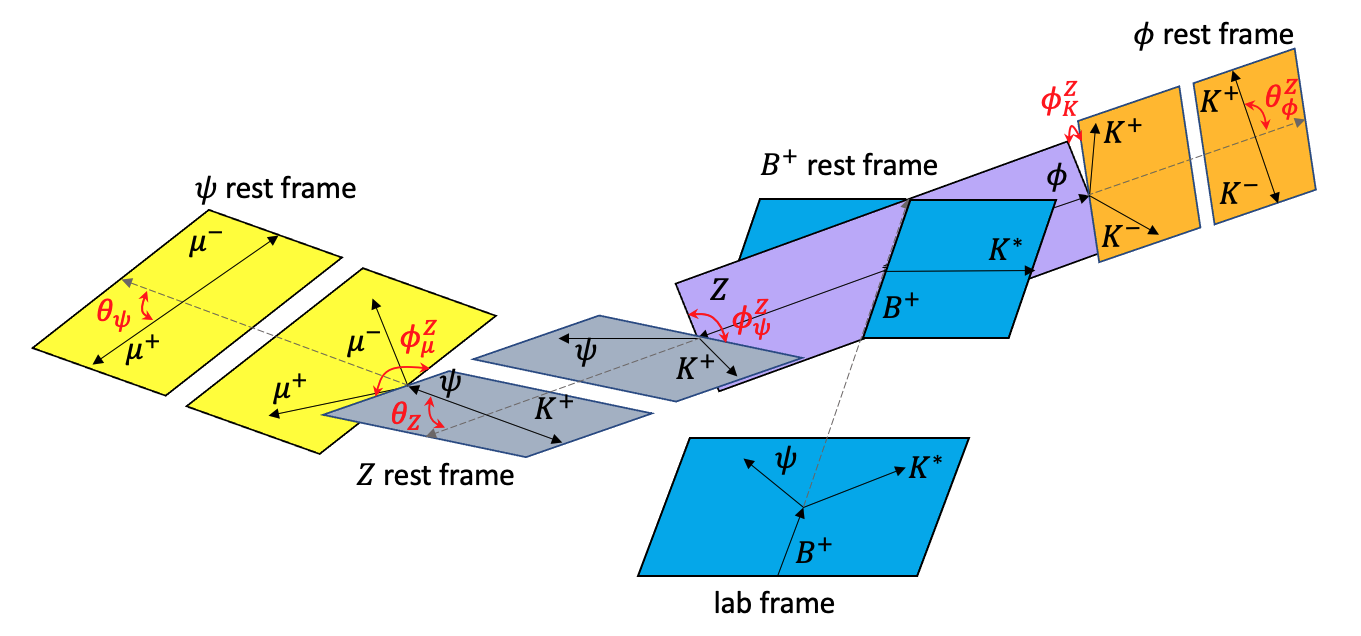
\includegraphics[width=0.95\textwidth]{Figures/05_Likelihood/Cartoon/B2ZPhi.png}%
   \caption{Defination of decay angles in the $Z^{+}$ chain.}
\label{fig:cartoon_chain_ZPhi}
\end{figure}

The angles used in $Z$ chain are defined in Fig.\ref{fig:cartoon_chain_ZPhi}.
The polar angle of $\phi$ in $Z$ rest frame can be calculated:
\begin{equation}
\cos \theta_{Z} = -\BA{\hat{p}}{\phi}{Z} \cdot \BA{\hat{p}}{\psi}{Z}
\end{equation}
The axis of $Z$ rest frame is defined as: 
\begin{align}
\BA{\hat{x}}{0}{Z} & = - \frac{\BA{\hat{p}}{\Bz}{LAB} - \left(\BA{\hat{p}}{\Bz}{LAB} \cdot \BA{\hat{p}}{Z}{\Bz} \right) \BA{\hat{p}}{Z}{\Bz} }  
{\left|\BA{\hat{p}}{\Bz}{LAB} - \left(\BA{\hat{p}}{\Bz}{LAB} \cdot \BA{\hat{p}}{Z}{\Bz} \right) \BA{\hat{p}}{Z}{\Bz}\right|}\\
\BA{\hat{y}}{0}{Z} &= - \BA{\hat{p}}{\phi}{Z} \times \BA{\hat{x}}{0}{Z}\\
\BA{\hat{z}}{0}{Z} & = - \BA{\hat{p}}{\phi}{Z}
\end{align}
The azimuthal angle of $\psi$ in $Z$ rest frame can be determined from:
\begin{equation}
\phi_{\psi}^{Z} = \mathrm{atan2}  \left( \BA{\hat{y}}{0}{Z} \cdot \BA{\hat{p}}{\psi}{Z} , \BA{\hat{x}}{0}{Z} \cdot \BA{\hat{p}}{\psi}{Z} \right)
\end{equation}
For the rest frame of $\phi$, the definition of axis:
\begin{align}
{\hat{x}}_{0}^{\{\phi\}Z} & = - \BA{\hat{x}}{0}{Z}\\
{\hat{y}}_{0}^{\{\phi\}Z} &= \BA{\hat{y}}{0}{Z}\\
{\hat{z}}_{0}^{\{\phi\}Z} & = - \BA{\hat{z}}{0}{Z}
\end{align}
The polar angle of $\Kp$ in $\phi$ rest frame:
\begin{equation}
\cos \theta_{\phi}^{Z} = -{\hat{p}}_{Z}^{\{\phi\}Z} \cdot {\hat{p}}_{\Kp}^{\{\phi\}Z}
\end{equation}
The azimuthal angle of $\Kp$ in $\phi$ rest frame:
\begin{equation}
\phi_{K}^{Z} = \mathrm{atan2}  \left( {\hat{y}}_{0}^{\{\phi\}Z} \cdot {\hat{p}}_{\Kp}^{\{\phi\}Z} , {\hat{x}}_{0}^{\{\phi\}Z} \cdot {\hat{p}}_{\Kp}^{\{\phi\}Z} \right)
\end{equation}
The definition of axis of $\psi$ rest frame is shown:
\begin{align}
{\hat{x}}_{0}^{\{\psi\}Z} & = - \frac{- \BA{\hat{p}}{\phi}{Z} + \left(\BA{\hat{p}}{\phi}{Z} \cdot \BA{\hat{p}}{\psi}{Z} \right) \BA{\hat{p}}{\psi}{Z} }  
{\left| - \BA{\hat{p}}{\phi}{Z} + \left(\BA{\hat{p}}{\phi}{Z} \cdot \BA{\hat{p}}{\psi}{Z} \right) \BA{\hat{p}}{\psi}{Z} \right|}\\
{\hat{y}}_{0}^{\{\psi\}Z} &= - {\hat{p}}_{\KS}^{\{\psi\}Z} \times {\hat{x}}_{0}^{\{\psi\}\Z}\\
{\hat{z}}_{0}^{\{\psi\}Z} & = - {\hat{p}}_{\KS}^{\{\psi\}Z}
\end{align}
The polar angle of $\mup$ in $\psi$ rest frame is defined as:
\begin{equation}
\cos \theta_{\psi}^{Z} = -{\hat{p}}_{\KS}^{\{\psi\}Z} \cdot {\hat{p}}_{\mup}^{\{\psi\}Z}
\end{equation}
The azimuthal angle of $\mup$ in $\psi$ rest frame:
\begin{equation}
\phi_{\mu}^{Z} = \mathrm{atan2}  \left(  {\hat{y}}_{0}^{\{\psi\}Z} \cdot {\hat{p}}_{\mup}^{\{\psi\}Z}, {\hat{x}}_{0}^{\{\psi\}Z} \cdot {\hat{p}}_{\mup}^{\{\psi\}Z} \right)
\end{equation}
The angle $\alpha_\mu^{Z}$ is defined as:
\begin{equation}
\alpha_\mu^{Z} = \mathrm{atan2}\left( \left(  \hat{z}_0^{\{\mup\}Z}  \times  \hat{x}_0^{\{\mup\}Z}  \right) \cdot \hat{x}_0^{\{\mup\}\Kstarz}, \hat{x}_0^{\{\mup\}Z}  \cdot \hat{x}_0^{\{\mup\}\Kstarz} \right)
\end{equation}
$\hat{z}_0^{\{\mup\}Z}$ means the z axis of $\mup$ rest frame in the $Z$ chain. Other symbols are similar. 
Here, $\hat{x}_0^{\{\mup\}\Kstarz}$, $\hat{x}_0^{\{\mup\}Z}$ and $\hat{x}_0^{\{\mup\}Z}$ are defined as:
\begin{align}
\label{Eq:app_axis_murest_in_kstar_chain}
\hat{x}_0^{\{\mup\}\Kstarz} & = 
- \frac{ -\hat{p}_{\Kstarz}^{\{\psi\}} + \left( \hat{p}_{\Kstarz}^{\{\psi\}} \cdot 
\hat{p}_{\mup}^{\{\psi\}} \right) 
\hat{p}_{\mup}^{\{\psi\}} }
{\left| -\hat{p}_{\Kstarz}^{\{\psi\}} + \left( \hat{p}_{\Kstarz}^{\{\psi\}} \cdot 
\hat{p}_{\mup}^{\{\psi\}} \right) 
\hat{p}_{\mup}^{\{\psi\}}  \right|}  \\%%%%%%%%
\hat{x}_0^{\{\mup\}Z} & = 
- \frac{ -\hat{p}_{\KS}^{\{\psi\}} + \left( \hat{p}_{\KS}^{\{\psi\}} \cdot 
\hat{p}_{\mup}^{\{\psi\}} \right) 
\hat{p}_{\mup}^{\{\psi\}} }
{\left| -\hat{p}_{\KS}^{\{\psi\}} + \left( \hat{p}_{\KS}^{\{\psi\}} \cdot 
\hat{p}_{\mup}^{\{\psi\}} \right) 
\hat{p}_{\mup}^{\{\psi\}}  \right|} \\ %%%%%%% 
\hat{z}_0^{\{\mup\}Z} & = \hat{p}_{\mup}^{\{\psi\}}
\end{align}
Keep in mind that the axes have to be calculated in the same $\psi$ rest frame.



\subsection{Matrix element for the $X \to \psi \phi$ chain}
The decay chain of $\Bp\to X_i \Kp$, $X_i\to \psi \phi$, $\phi\to K^+K^-$,  $\psi\to \mu^+\mu^-$ also contains four terms. 
The $\Bs\to X_i \Kp$ gives a constant term $\H^{\Bp\to X_i \Kp}$ and limits $\lambda_{X}=\lambda_{K}^X=0$. 

The $X_i \to \psi \phi$ is described by the term 
\begin{equation}
\H_{\lambda_\psi^{X},\lambda_\phi^X}^{X_{i}}D^{\,\,J_{X_i}}_{0,\,\lambda_\psi^{X}-\lambda_\phi^X}(\phi_\psi^X,\theta_{X},0)^*R_{X_i}(m_{\psi \phi}),
\end{equation}
The helicity angles of $X$ decays $\phi_\psi^X$ and $\theta_{X}$ are defined by the $\psi$ direction. 
The strong decay conserves parity, which gives the relation $\H_{-\lambda_\psi^{X},-\lambda_\phi^{X}}^{X}=(-1)^{J_{X}}P_{X_j}\H_{\lambda_\psi^{X},\lambda_\phi^{X}}^{X}$.

The $\phi\to K^+K^-$ provides one term 
\begin{equation}
D^{\,\,1}_{\lambda^X_{\phi},\,0}(\phi^X_{K^+},\theta^X_\phi,0)^*,
\end{equation}
where $K^+$ is used to define the two helicity angles of $\phi^X_{K^+}$ and $\theta^X_\phi$ from $\phi$ decays. 
We use the superscript $X$ to differentiate from the other decay chains. 

The $\psi\to\mu^+\mu^-$ decay is described by the term
\begin{equation}
D^{\,\,1}_{\lambda^{X}_{\psi},\,\Delta\lambda^{X}_\mu}(
\phi_{\mu}^{X},\theta_{\psi}^{X},0)^*.
\end{equation}
The muon helicity states are aligned by $\alpha^X_\mu$ rotation.

The total matrix element for the $X$ chain from $\Bp$ decay is 
\begin{align}
{\Mat}^X_{\Delta\lambda_\mu}&(\theta_{X},\theta_\psi^{X},\theta_\phi^X, \phi_{K^+}^X,\phi_\mu^{X},\alpha^{X}_\mu,m_{\psi\phi})=e^{i\Delta\lambda_\mu\alpha^{X}_{\mu}} \sum\limits_{\lambda_\psi^{X}}e^{i \lambda^{X}_{\psi} \phi_{\mu}^{X}}d^{\,\,1}_{\lambda^{X}_{\psi},\,\Delta\lambda_\mu}(\theta_{\psi}^{X})  \notag\\
&\times \sum\limits_{\lambda^X_{\phi}}e^{i\lambda^X_{\phi} \phi^X_{K^+}} d^{\,\,1}_{\lambda^X_{\phi},\,0}(\theta^X_\phi) 
\sum\limits_{i}\H^{\Bp\to X_i \Kp}\H_{\lambda_\psi^{X},\lambda_\phi^X}^{X_{i}} d^{\,\,J_{X_i}}_{0,\,\lambda_\psi^{X}-\lambda_\phi^X}(\theta_{X})R_{X_i}(m_{\psi \phi}).
\end{align}
%Here the relation $\Delta\lambda^{X}_\mu=\Delta\lambda_\mu$ is applied. ????

\begin{figure}[!hbtp]
\centering
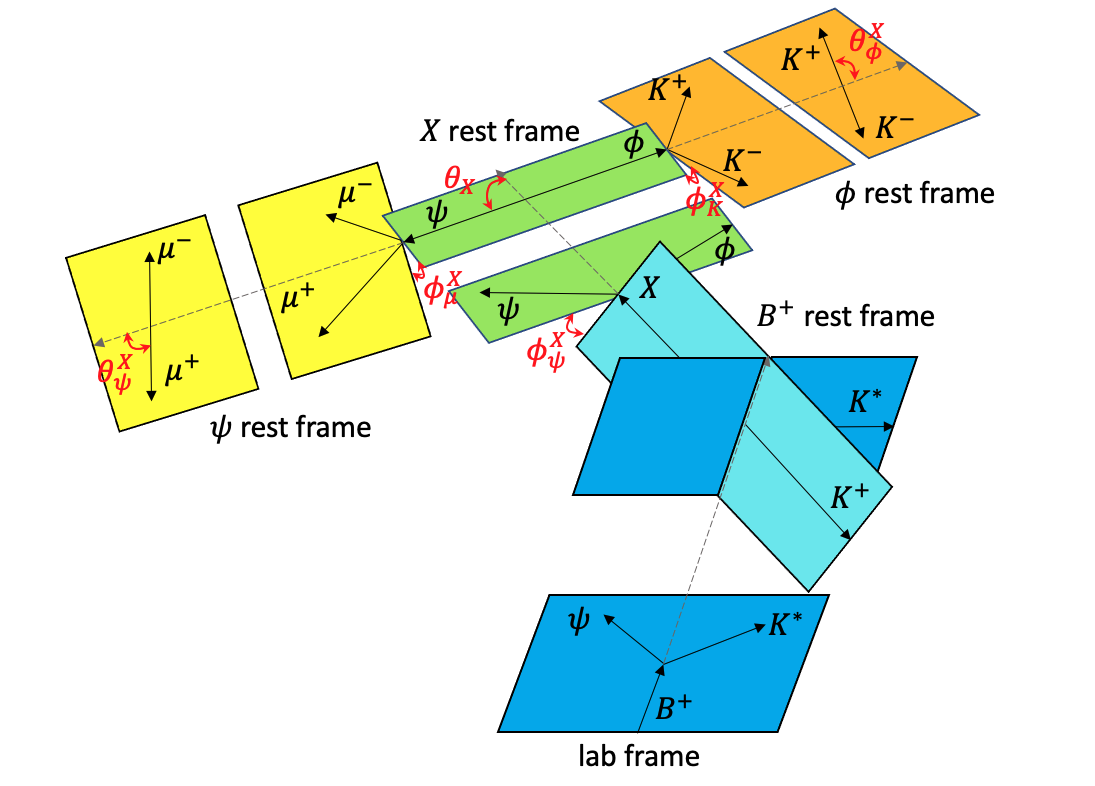
\includegraphics[width=0.95\textwidth]{Figures/05_Likelihood/Cartoon/B2XK.png}%
   \caption{Defination of decay angles in the $X$ chain.}
\label{fig:cartoon_chain_XK}
\end{figure}

The angles used in $X$ chain are defined in Fig.\ref{fig:cartoon_chain_XK}.
The polar angle of $\psi$ in $X$ rest frame can be calculated:
\begin{equation}
\cos \theta_{X} = -\BA{\hat{p}}{\KS}{X} \cdot \BA{\hat{p}}{\psi}{X}
\end{equation}
The axis of $X$ rest frame is defined as: 
\begin{align}
\BA{\hat{x}}{0}{X} & = - \frac{\BA{\hat{p}}{\Bz}{LAB} - \left(\BA{\hat{p}}{\Bz}{LAB} \cdot \BA{\hat{p}}{X}{\Bz} \right) \BA{\hat{p}}{X}{\Bz} }  
{\left|\BA{\hat{p}}{\Bz}{LAB} - \left(\BA{\hat{p}}{\Bz}{LAB} \cdot \BA{\hat{p}}{X}{\Bz} \right) \BA{\hat{p}}{X}{\Bz}\right|}\\
\BA{\hat{y}}{0}{X} &= - \BA{\hat{p}}{\KS}{X} \times \BA{\hat{x}}{0}{X}\\
\BA{\hat{z}}{0}{X} & = - \BA{\hat{p}}{\KS}{X}
\end{align}
The azimuthal angle of $\psi$ in $X$ rest frame can be determined from:
\begin{equation}
\phi_{\psi}^{X} = \mathrm{atan2}  \left( \BA{\hat{y}}{0}{X} \cdot \BA{\hat{p}}{\psi}{X} , \BA{\hat{x}}{0}{X} \cdot \BA{\hat{p}}{\psi}{X} \right)
\end{equation}
The definition of axis of $\psi$ rest frame is shown:
\begin{align}
{\hat{x}}_{0}^{\{\psi\}X} & = - \frac{- \BA{\hat{p}}{\KS}{X} + \left(\BA{\hat{p}}{\KS}{X} \cdot \BA{\hat{p}}{\psi}{X} \right) \BA{\hat{p}}{\psi}{X} }  
{\left| - \BA{\hat{p}}{\KS}{X} + \left(\BA{\hat{p}}{\KS}{X} \cdot \BA{\hat{p}}{\psi}{X} \right) \BA{\hat{p}}{\psi}{X} \right|}\\
{\hat{y}}_{0}^{\{\psi\}X} &= - {\hat{p}}_{\phi}^{\{\psi\}X} \times {\hat{x}}_{0}^{\{\psi\}X}\\
{\hat{z}}_{0}^{\{\psi\}X} & = - {\hat{p}}_{\phi}^{\{\psi\}X}
\end{align}
The polar angle of $\mup$ in $\psi$ rest frame is defined as:
\begin{equation}
\cos \theta_{\psi}^{X} = -{\hat{p}}_{\phi}^{\{\psi\}X} \cdot {\hat{p}}_{\mup}^{\{\psi\}X}
\end{equation}
The azimuthal angle of $\mup$ in $\psi$ rest frame:
\begin{equation}
\phi_{\mu}^{X} = \mathrm{atan2}  \left(  \BA{\hat{y}}{0}{\psi} \cdot \BA{\hat{p}}{\mup}{\psi}, \BA{\hat{x}}{0}{\psi} \cdot \BA{\hat{p}}{\mup}{\psi} \right)
\end{equation}
The angle $\alpha_\mu^X$ is defined as:
\begin{equation}
\alpha_\mu^X = \mathrm{atan2}\left( \left(  \hat{z}_0^{\{\mup\}X}  \times  \hat{x}_0^{\{\mup\}X}  \right) \cdot \hat{x}_0^{\{\mup\}\Kstarz}, \hat{x}_0^{\{\mup\}X}  \cdot \hat{x}_0^{\{\mup\}\Kstarz} \right)
\end{equation}
$\hat{z}_0^{\{\mup\}X}$ means the z axis of $\mup$ rest frame in the $X$ chain. Other symbols are similar. 
Here, $\hat{x}_0^{\{\mup\}\Kstarz}$ is defined in Eq.\ref{Eq:app_axis_murest_in_kstar_chain}, $\hat{x}_0^{\{\mup\}X}$ and $\hat{x}_0^{\{\mup\}X}$ are defined as:
\begin{align}
\hat{x}_0^{\{\mup\}X} & = 
- \frac{ -\hat{p}_{\phi}^{\{\psi\}} + \left( \hat{p}_{\phi}^{\{\psi\}} \cdot 
\hat{p}_{\mup}^{\{\psi\}} \right) 
\hat{p}_{\mup}^{\{\psi\}} }
{\left| -\hat{p}_{\phi}^{\{\psi\}} + \left( \hat{p}_{\phi}^{\{\psi\}} \cdot 
\hat{p}_{\mup}^{\{\psi\}} \right) 
\hat{p}_{\mup}^{\{\psi\}}  \right|} \\ %%%%%%% 
\hat{z}_0^{\{\mup\}X} & = \hat{p}_{\mup}^{\{\psi\}}
\end{align}

For the rest frame of $\phi$, the definition of axis:
\begin{align}
\hat{x}_{0}^{\{\phi\} X} & = - \BA{\hat{x}}{0}{X}\\
\hat{y}_{0}^{\{\phi\} X} &= \BA{\hat{y}}{0}{X}\\
\hat{z}_{0}^{\{\phi\} X} & = - \BA{\hat{z}}{0}{X}
\end{align}
The polar angle of $\Kp$ in $\phi$ rest frame:
\begin{equation}
\cos \theta_{\phi}^{X} = -\hat{p}_{\psi}^{\{\phi\}X} \cdot \hat{p}_{\Kp}^{\{\phi\}X}
\end{equation}
The azimuthal angle of $\Kp$ in $\phi$ rest frame:
\begin{equation}
\phi_{K}^{X} = \mathrm{atan2}  \left( \hat{y}_{0}^{\{\phi\}X} \cdot {\hat{p}}_{\Kp}^{\{\phi\}X} , {\hat{x}}_{0}^{\{\phi\}X} \cdot {\hat{p}}_{\Kp}^{\{\phi\}X} \right)
\end{equation}

Finally, total matrix element squared is given by
\begin{equation} 
\left| \Mat \right|^2  = 
\sum\limits_{\Delta\lambda_{\mu}=\pm1}
\left|
\Mat_{\Delta\lambda_\mu}^{\Kst} 
+ 
\Mat_{\Delta\lambda_\mu}^{Z}  
+ \Mat_{\Delta\lambda_\mu}^{X} 
\right|^2
\label{SUPPeq:total_matrixelement}
\end{equation}  

Assuming approximate $\CP$ symmetry, the helicity couplings for $\Bp$ and $\Bm$ can be made equal, 
but the calculation of the angles requires some care, 
since parity ($P$) conservation does not change polar (i.e. helicity) angles, 
but does change azimuthal angles. 
Thus, not only must $\vec{p}_{\mu^-}$ be used instead of $\vec{p}_{\mu^+}$ for $\Bm$ candidates, 
as well as $K^-$ instead of $K^+$ for the $\phi$ decay,  
but also all azimuthal angles must be reflected before entering the matrix element formula:
all $\phi_{i}\to -\phi_{i}$,  
and 
two $\alpha_\mu\to -\alpha_\mu$
\cite{Chilikin:2013tch}.


\subsection{Usage of $LS$ couplings}

Since not all helicity couplings are independent because of parity conservation in strong decays, 
it is convenient to related them to the $LS$ couplings ($B_{L,S}$) using Clebsch-Gordan coefficients
\begin{equation}
\H_{\lambda_B,\lambda_C}^{A\to B\,C}=\sum_{L} \sum_{S} 
\sqrt{ \tfrac{2L+1}{2J_A+1} } B_{L,S} 
\left( 
\begin{array}{cc|c}
 J_{B} & J_{C} & S \\
 \lambda_{B} & -\lambda_{C} & \lambda_{B}-\lambda_{C} 
\end{array}
\right)
\times
\left( 
\begin{array}{cc|c}
 L  & S & J_A \\
 0 & \lambda_{B}-\lambda_{C} & \lambda_{B}-\lambda_{C}   
\end{array}
\right). 
\label{SUPeq:LS}
\end{equation}
Here $L$ is the orbital angular momentum in the decay, and 
$S$ is the total spin of the daughters, $\vec{S}=\vec{J}_B+\vec{J}_C$
($|J_B-J_C|\le S \le J_B+J_C$).
The $LS$ couplings are all independent since they automatically satisfy the parity conservation relation in strong decays, 
by restricting $L$ value to be odd or even using the selection $P_A=(-1)^L P_B \cdot P_C$, where $P$ is parity of the particle.   

Table~\ref{tab:KLS} shows the allowed $LS$ for various $J^P$ of $K$ excitations. 
The rule also applies to the $Z\to\psi K$ chain, 
because $\psi$ and $\phi$ are vector particles, 
have the same $J^P=1^-$.
For $\Bp\to \psi K^*_n$ decays, $S=L_{B}^{K^*_n}$ can have up to three values, 
$J_{K^*_n}-1$, $J_{K^*_n}$ and $J_{K^*_n}+1$ (except for when $J_{K^*_n}=0$, 
only one value $L_{B}^{K^*_n}=1$ is possible), corresponding to three (or one) $B^{\Bp\to \psi K^*_n}_{L,S}$ couplings, respectively. 
For $K^*_n\to \phi K$ decay, $S=1$, and $|J_{K^*_n}-1|\le L_{K^*_n} \le J_{K^*_n}+1$. 
Again when $J_{K^*_n}=0$, $L_{K^*_n}=1$. 
Parity conservation limits $L_{K^*_n}$ to be even or odd by $P_{K^*_n}=(-1)^{L_{K^*_n}}$, 
and natural parity ($1^-$, $2^+$, $0^+$ is forbidden) allows one $L_{K^*_n}$, 
while unnatural parity ($1^+$, $2^-$ ...) allows two $L_{K^*_n}$.  
Since only the product of $\Bp$ and $K^*_n$ couplings can be determined, 
lowest $L_{\rm min}$ coupling of $K^*$ decay $B^{K^*_n\to \phi K}_{L_{\rm min},S}$ is defined as $(1,0)$,
which reduces one free coupling. 
To summarize whole $K^*$ decay chain,  
$0^+$ ${K^*_n}$ is forbidden, 
$0^-$ is described by one coupling, $1^-$, $2^+$ ... by three couplings, and $1^+$, $2^-$ ... by four couplings.  
The $0^-$  $\nslj{2}{1}{S}{0}$ is chosen as the reference channel, 
and the only one coupling of $B$ decay is fixed to be $(1,0)$.  
This is a very good choice to make fit stable, 
since the state has large and stable fit fraction about 10\%, 
and only-one coupling is directly proportional to its fit fraction. 

For $\Bp\to X_i \Kp$ decays, 
only one coupling is needed, 
the coupling $B^{\Bp\to X_i \Kp}$ is equal to $(1,0)$, 
again because only the product of $\Bp$ and $X_i$ couplings can be determined.  
For $X_i\to \psi \phi$ decays, $S=0,1,2$ and parity conservation relation $P_{X_i}=(-1)^{L_{X_i}}$  reduces $L_{X_i}$ to about half. 
Table~\ref{tab:XLS} shows the allowed $LS$ for various $J^P$ of $X_i$. 
Each $LS$ combination requires one coupling that are determined by the fit.


\begin{table}[!hbtp]
\caption{Allowed $LS$ for various $J^P$ in the $K^*_n \to \phi K$ decay chain.}\label{tab:KLS}
\centering
\begin{tabular}{c|l|l}
$J^P$& $K^*_n \to \phi K$ & $B\to \jpsi K_n^*$ \\\hline
$0^+$& forbidden&-\\
$0^-$& 11 &11\\
$1^+$& 01, 21 &00, 11, 22\\
$1^-$ & 11 &00, 11, 22\\
$2^+$ & 21 &11, 22, 33\\
$2^-$ & 11, 31 &11, 22, 33\\
\end{tabular}
\end{table}

\begin{table}[!hbtp]
\caption{Allowed $LS$ for various $J^P$ in the $X\to\jpsi \phi$ decay chain.}\label{tab:XLS}
\centering
\begin{tabular}{c|l|l}
$J^P$& $X_i\to \jpsi \phi$& $B\to X_i K$ \\\hline
$0^+$& $00$, $22$&00\\
$0^-$& $11$&00\\
$1^+$& $01$, $21$, $22$&11\\
$1^-$ & $10$, $11$, $12$, $32$&11\\
$2^+$ & $02$, $20$, $21$, $22$, $42$&22\\
$2^-$ & $11$, $12$, $31$, $32$&22\\
\end{tabular}
\end{table}




\subsection{$cFit$ technique}

We use cFit technique used in the previous publication~\cite{LHCb-PAPER-2016-018}, which contains both signal and background PDFs.
The signal PDF, $\PDF_{\rm sig}$,
is proportional to the matrix element squared, which 
is a function of six independent variables: 
$m_{\phi K}$ 
and the independent angular variables in the $\Kstar$ decay chain $\Omega$. 
%
The PDF also depends on the fit parameters, $\Pars$, which include the 
helicity couplings, and masses and widths of resonances. 
%
The two other invariant masses, $m_{\phi K}$ and $m_{\jpsi K}$, and 
the angular variables describing the $X$ and $Z_{cs}^+$ decay chains 
depend on $m_{\phi K}$ and $\Omega$, therefore they do not represent independent dimensions. 
%
The signal PDF is given by:
\begin{equation}
\label{eq:sigpdfsplot}
\frac{d\PDF}{d m_{\phi K}\,d\Omega} \equiv \PDF_{\rm sig}(m_{\phi K},\Omega|\Pars)
=\frac{1}{I(\overrightarrow{w})}\big|\Mat(m_{\phi K},\Omega| \Pars)\big|^2
\Phi(m_{\phi K})
\epsilon(m_{\phi K},\Omega),
\end{equation}
where $\Mat(m_{\phi K},\Omega|\Pars)$ is the total matrix element given by Eq.~(\ref{SUPPeq:total_matrixelement}) and discussed in detail in Appendix~\ref{SUPPsec:matrixelement}. 
$\Phi(m_{\phi K})=p\,q$ is the phase space function, where $p$ is the momentum of
the $\phi K^+$ (\ie $\Kstar$) system in the $B^+$ rest frame, and $q$ is the $K^+$ momentum 
in the $K^{*+}$ rest frame.
The function $\epsilon(m_{\phi K},\Omega)$ is the signal efficiency, and
$I(\Pars)$ is the normalization integral,
\begin{equation}
I(\Pars)\equiv \int \PDF_{\rm sig}(m_{\phi K},\Omega)\,d m_{\phi K}\,d\Omega \propto
\frac{\sum_j w_j^{\rm MC}\big|\Mat(m_{Kp~j},\Omega_j|\Pars)\big|^2}{\sum_j w_j^{\rm MC}},
\label{eq:signor}
\end{equation}
where the sum is over simulated events, which are
generated uniformly in $B^+$ decay phase space 
and passed through the detector simulation \cite{LHCb-PROC-2011-006}
and data selection.
In the simulation, $pp$ collisions producing $B^+$ mesons are generated using
\pythia~\cite{Sjostrand:2006za}  with a specific \lhcb
configuration~\cite{LHCb-PROC-2010-056}. 
The weights $w_j^{\rm MC}$ introduced in Eq.~(\ref{eq:signor}) contain 
corrections to the $B^+$ production kinematics and multiplicity in the generation 
and to the detector response 
to bring the simulations into better agreement with the data.
The simulation sample contains 390\,000 events reconstructed and selected,
approximately 15 times the signal size in data. Run1 MC $w_j^{\rm MC}$ is multiplied by a constant 
scale (about 0.5) to let the sum of weights is proportional to the signal yield found in data, \ie the ratio of MC sum weights is
the same as the ratio of signal yields in Run 1 and Run 2 data.
This procedure folds the detector response into the model 
and allows a direct determination of the parameters of interest from the uncorrected data. 
The resulting log-likelihood 
sums over the data events (here for illustration, $\PDF=\PDF_{\rm sig}$),
{%
\def\1{\ifthenelse{\boolean{prl}}{}{\!\!}}
\begin{equation}
\begin{split}
\ln L(\Pars) & = \sum_i \ln \PDF_{\rm sig}(m_{\phi K~i},\Omega_i|\Pars)  \\%\notag\\
 & = \sum_i \ln \big|\Mat(m_{\phi K~i},\Omega_i|\Pars)\big|^2  - N\ln I(\Pars) + \sum_i \ln[ \Phi(m_{\phi K~i})\epsilon(m_{\phi K~i},\Omega_i) ],
\end{split}
\end{equation}
}%
where the last term does not depend on $\Pars$ and can be dropped ($N$ is the total number of the events in the fit).   

In addition to the signal PDF, $\PDF_{\rm sig}(m_{\phi K},\Omega|\Pars)$,
the background PDF, $\PDF_{\rm bkg}(m_{\phi K},\Omega)$ 
determined from the $B^+$ mass peak sidebands, is included.
%
We minimize the negative log-likelihood defined as
\begin{equation}
\begin{split}
& -\ln L(\Pars)=
-\sum_i\ln \left[ (1-\beta)\, \PDF_{\rm sig}(m_{\phi K~i},\Omega_i|\Pars)
    + \beta\, \PDF_{\rm bkg}(m_{\phi K~i},\Omega_i) \right] \\%\nonumber \\
&=-\sum_i\ln \left[ (1-\beta)\,\frac{\big|\Mat(m_{\phi K~i},\Omega_i|\Pars)\big|^2 \Phi(m_{\phi K~i})\epsilon(m_{\phi K~i},\Omega_i)}{I(\Pars)}
+\beta\, \frac{\PDF_{\rm bkg}^{u}(m_{\phi K~i},\Omega_i)}{I_{\rm bkg}} \right] \\%\nonumber \\
%&=-\sum_i\ln \left\{ \frac{(1-\beta)\,\Phi(m_{\phi K~i})\epsilon(m_{\phi K~i},\Omega_i)}{I(\Pars)}\,\left[\big|\Mat(m_{\phi K~i},\Omega_i|\Pars)\big|^2 
%\right.\right. 
%\nonumber\\
%& \quad\quad\quad\quad\quad\quad\quad\quad\quad\quad\quad\quad\quad\quad\quad\quad\quad\quad\quad\quad \left.\left.
%+ \frac{\beta\,I(\Pars)}{(1-\beta)\,I_{\rm bkg}}\, \frac{\PDF_{\rm bkg}^{u}(m_{\phi K~i},\Omega_i)}{\Phi(m_{\phi K~i})\epsilon(m_{\phi K~i},\Omega_i)} 
%\right] \right\} \\%\nonumber \\
&=-\sum_i\ln \left[\big|\Mat(m_{\phi K~i},\Omega_i|\Pars)\big|^2  
+ \frac{\beta\,I(\Pars)}{(1-\beta) I_{\rm bkg}}\,\frac{\PDF_{\rm bkg}^{u}(m_{\phi K~i},\Omega_i)}{\Phi(m_{\phi K~i})\epsilon(m_{\phi K~i},\Omega_i)}\right]
+N\ln I(\Pars)+{\rm const.},
\end{split}
\end{equation}
where $\beta$ is the background fraction in the peak region determined from the fit to
the $m_{\jpsi \phi K}$ distribution (Fig.~\ref{fig:MassFit_run}), 
$\PDF_{\rm bkg}^{u}(m_{\phi K},\Omega)$ is the unnormalized background density proportional to the density of sideband events,
with its normalization determined by\footnote{Notice that the distribution of MC events 
includes both the $\Phi(m_{\phi K})$ and $\epsilon(m_{\phi K},\Omega)$ factors, which cancel their product in the numerator.}
\begin{equation}
I_{\rm bkg}\equiv \int \PDF_{\rm bkg}^{u}(m_{\phi K})\,d m_{\phi K}\,d\Omega \, \propto \,
\frac{
\sum_j w_j^{\rm MC} \frac{\PDF_{\rm bkg}^{u}(m_{\phi K~j},\Omega_j)}{\Phi(m_{\phi K~i})\epsilon(m_{\phi K~j},\Omega_j)}}{
\sum_j w_j^{\rm MC}}.
\label{eq:bkgnor}
\end{equation}
The equation above implies that the background term is efficiency corrected,
so it can be added
to the efficiency-independent signal probability expressed by $\left|\Mat\right|^2$.
This way the efficiency parameterization, $\epsilon(m_{\phi K},\Omega)$, 
becomes a part of the background description which affects only a very small part 
of the total PDF.

The efficiency parameterization
in the background term is assumed to factorize as
\begin{equation}
\begin{split}
\lefteqn{\epsilon(m_{\phi K},\Omega)=\epsilon_1(m_{\phi K},\cosks)\,\,\epsilon_2(\cosphi|m_{\phi K})\times} \\%\notag\\
&\quad\quad\quad\quad \epsilon_3(\cospsi|m_{\phi K})\,\, \epsilon_4(\phiksphi|m_{\phi K})\,\,\epsilon_5(\phikspsi|m_{\phi K}).
\end{split}
\label{eq:peff}
\end{equation}
The $\epsilon_1(m_{\phi K},\cosks)$ term is obtained by binning 
a two-dimensional (2D) histogram of the simulated signal events. 
Each event is given a $1/(p\,q)$ weight, 
since at the generator level the phase space is flat in $\cosks$ 
but has a $p\,q$ dependence on $m_{\phi K}$.
A bi-cubic function is used to interpolate between bin centers.
The $\epsilon_1(m_{\phi K},\cosks)$ efficiency and
its visualization across the normal Dalitz plane are shown in Fig.~\ref{fig:effm}.
The other terms are again built from 2D histograms, 
but with each bin divided by the number of simulated events in the corresponding 
$m_{\phi K}$ slice to remove the dependence on this mass (Fig.~\ref{fig:effepsilon2345}).

\begin{figure}[tbhp]
  \begin{center}
   % \includegraphics*[width=\figsize]{effm1cosKs.pdf} \\
    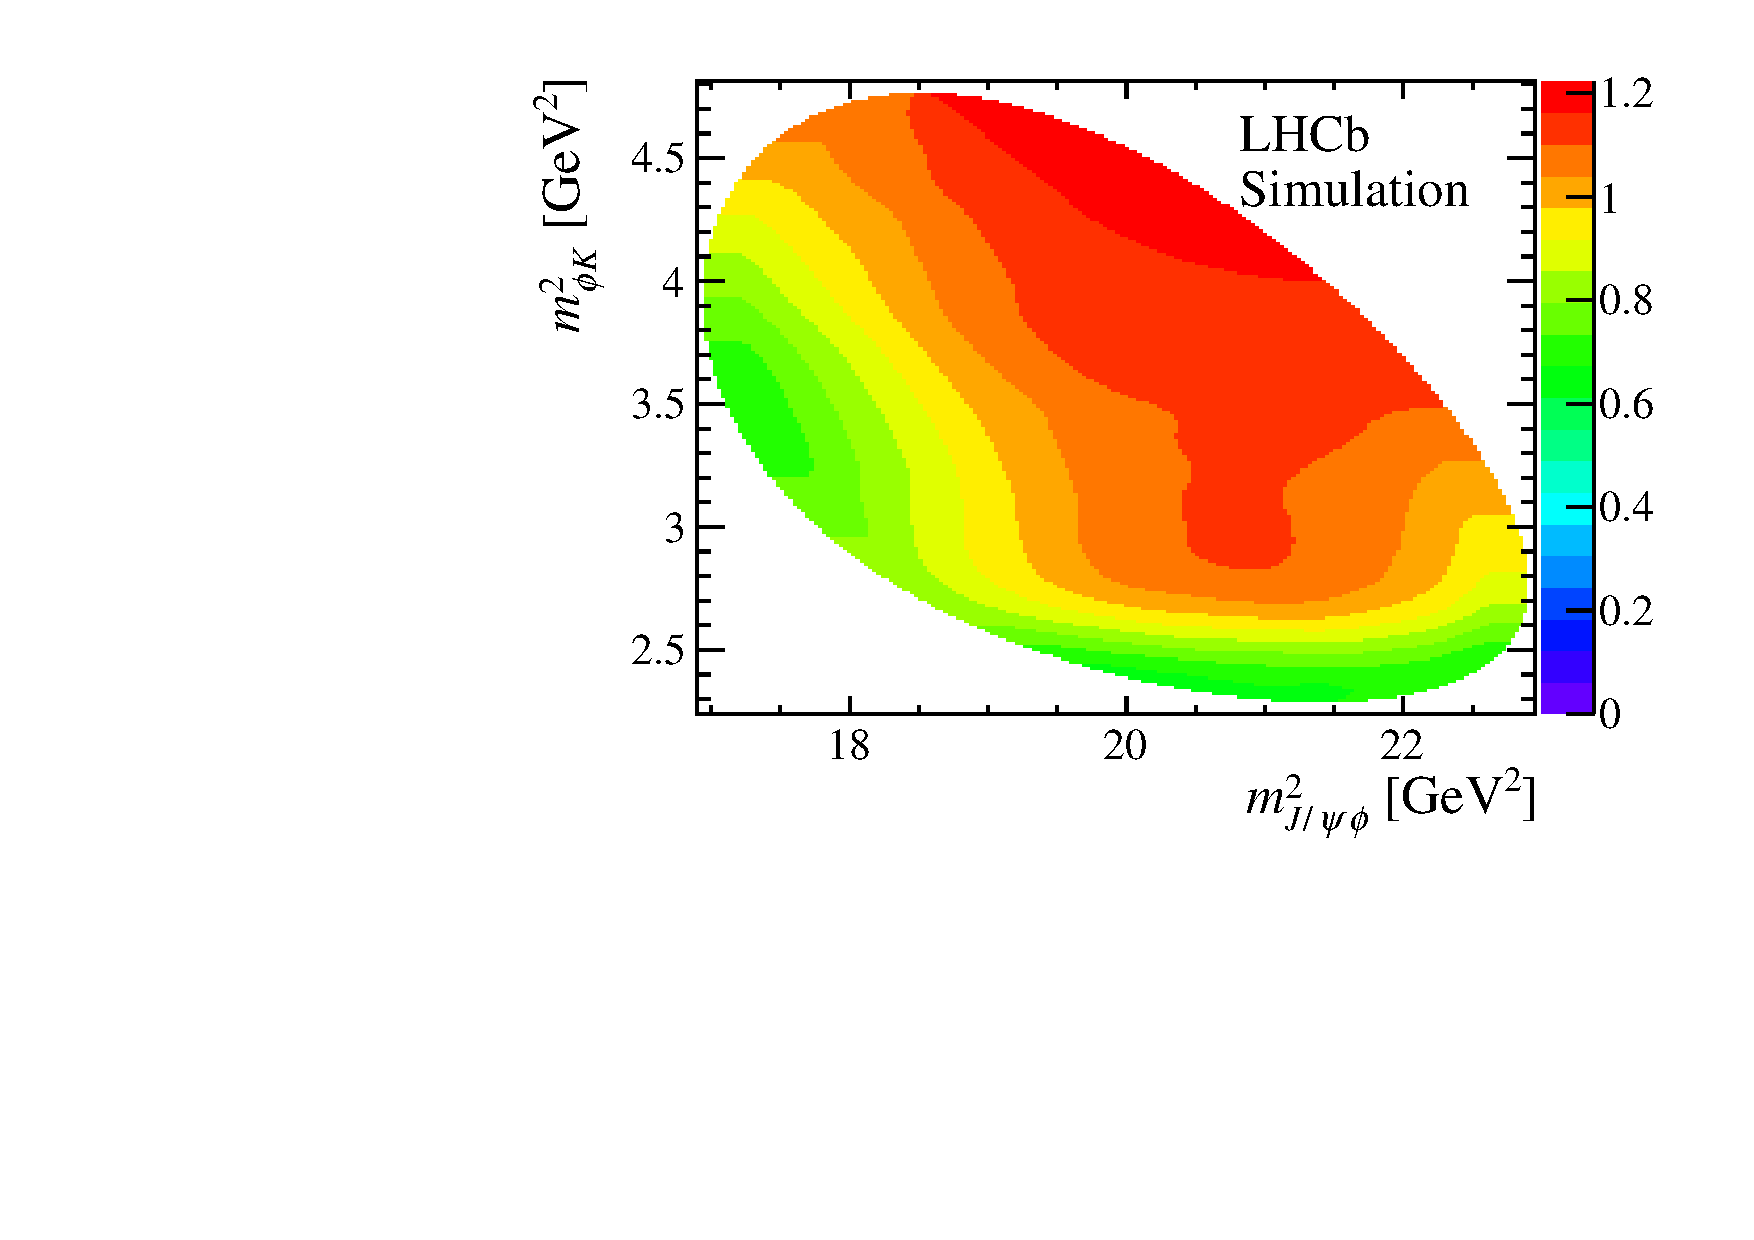
\includegraphics[width=0.8\textwidth]{Figures/05_Likelihood/effm1m2}
  \end{center}
  \vskip-0.3cm\caption{
     Parameterized efficiency representation in the Dalitz plane $({\mjpsiphi^2}, {\mphik^2})$.
     Function values corresponding to the color encoding are given on the right.
     The normalization arbitrarily corresponds to unity when averaged over the phase space.     
  \label{fig:effm}
  }
\end{figure}

\begin{figure}[bthp]
  \begin{center}
    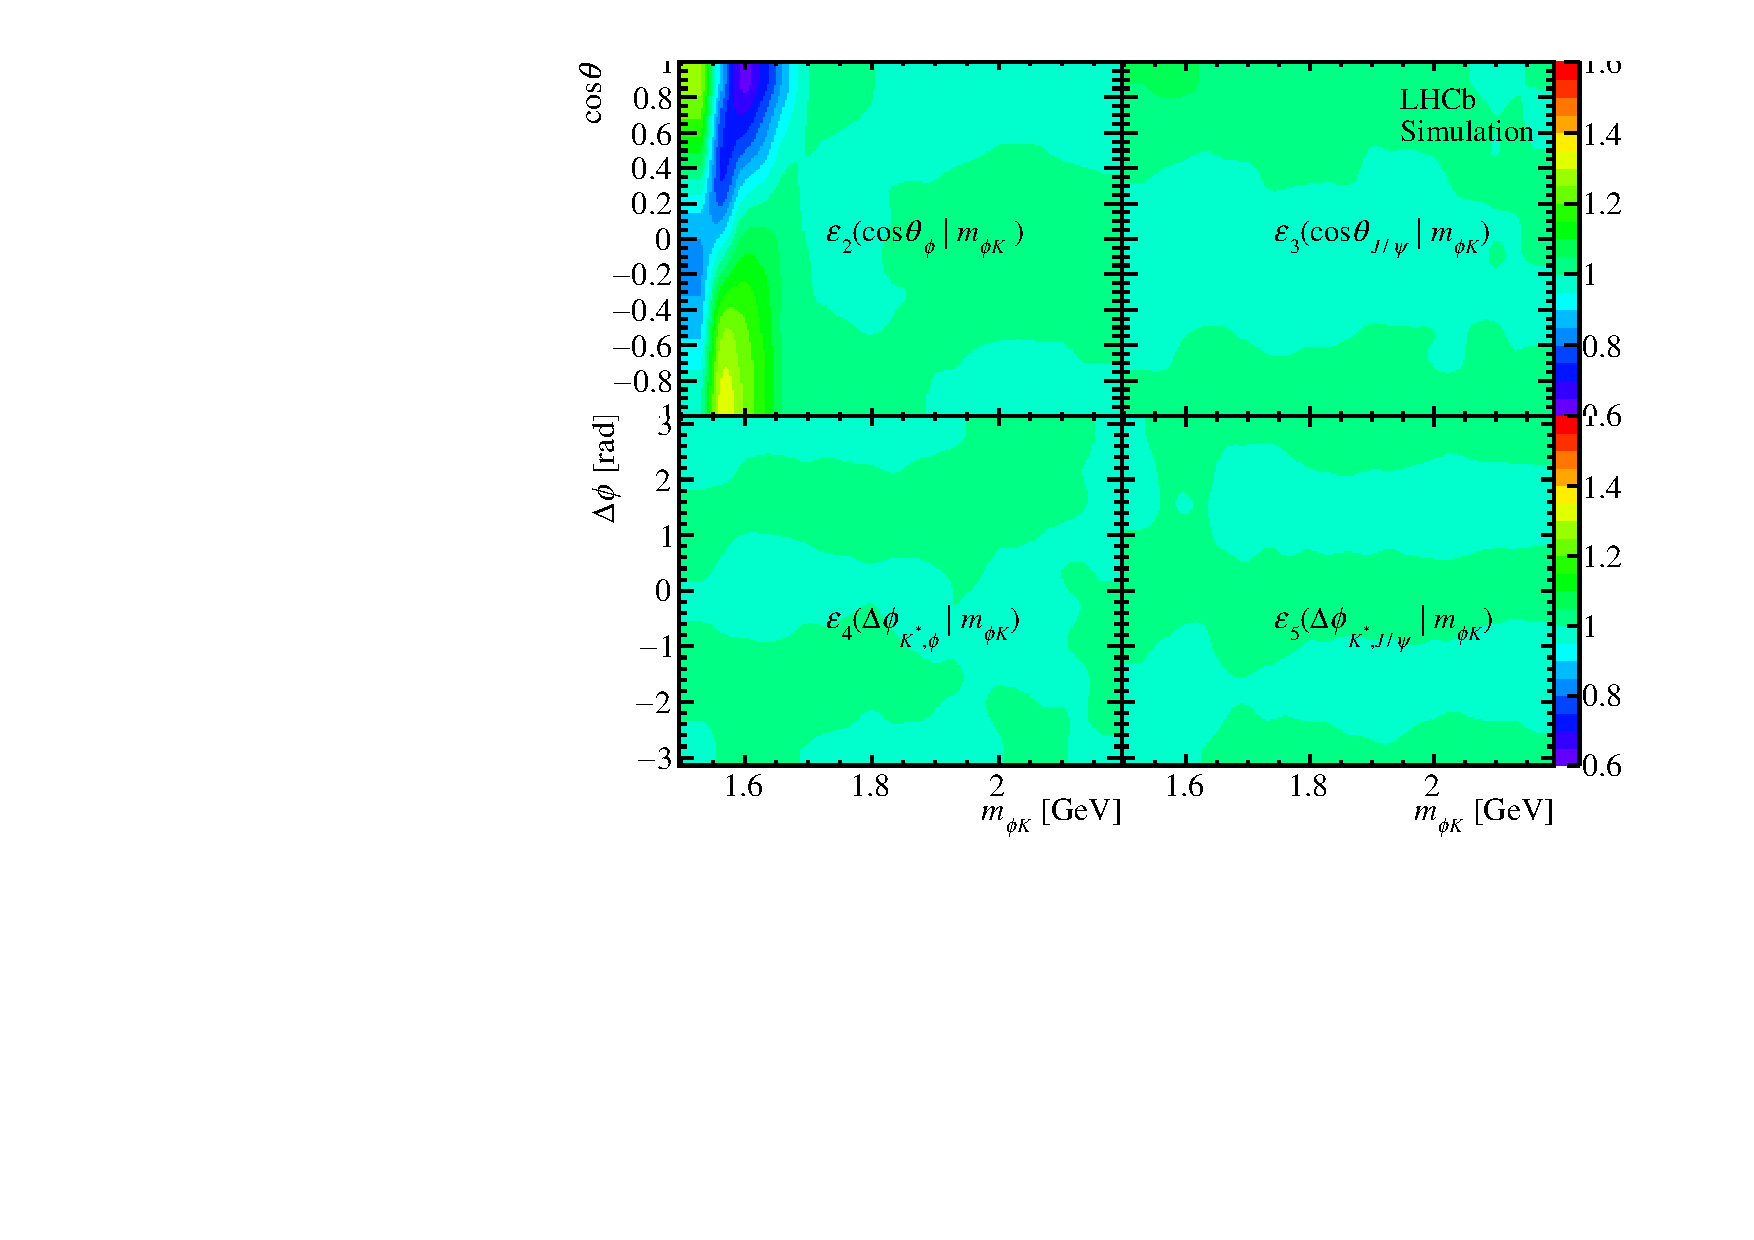
\includegraphics[width=0.8\textwidth]{Figures/05_Likelihood/effAngles} 
  \end{center}
  \vskip-0.3cm\caption{\small
     Parameterized efficiency 
     $\epsilon_2(\cosphi|m_{\phi K})$, $\epsilon_3(\cospsi|m_{\phi K})$,  
     $\epsilon_4(\phiksphi|m_{\phi K})$, $\epsilon_5(\phikspsi|m_{\phi K})$
     functions.
     Function values corresponding to the color encoding are given on the right.
     By construction each function integrates to unity at each $m_{\phi K}$ value.  
     The structure in $\epsilon_2(\cosphi|m_{\phi K})$ present 
     between 1500 and $1600 \mev$ is an artifact of 
     removing $\Bp \to \jpsi K^+ K^- K^+$ events in which both $K^+K^-$ combinations 
     pass the $\phi$ mass selection window. 
  }\label{fig:effepsilon2345}
\end{figure}

The background PDF, $\PDF_{\rm bkg}^{u}(m_{\phi K},\Omega)/\Phi(m_{\phi K})$, 
is built using the same approach,
\begin{equation}
\begin{split}
\lefteqn{
\frac{{\PDF_{\rm bkg}^{u}}(m_{\phi K},\Omega)}{\Phi(m_{\phi K})}=
{P_{\rm bkg}}_1(m_{\phi K},\cosks)\,\,{P_{\rm bkg}}_2(\cosphi|m_{\phi K})\times}
\\%\notag\\
&\quad\quad\quad{P_{\rm bkg}}_3(\cospsi|m_{\phi K})\,\, {P_{\rm bkg}}_4(\phiksphi|m_{\phi K})\,\,{P_{\rm bkg}}_5(\phikspsi|m_{\phi K}).
\end{split}
\label{eq:pbkg}
\end{equation}
The background function ${P_{\rm bkg}}_1(m_{\phi K},\cos\theta_\Kstar)$ is 
shown in Fig.~\ref{fig:bkgdaleffs} and the other terms are shown in 
Fig.~\ref{fig:bkgeffs2345}.

\begin{figure}[bthp]
  \begin{center}
    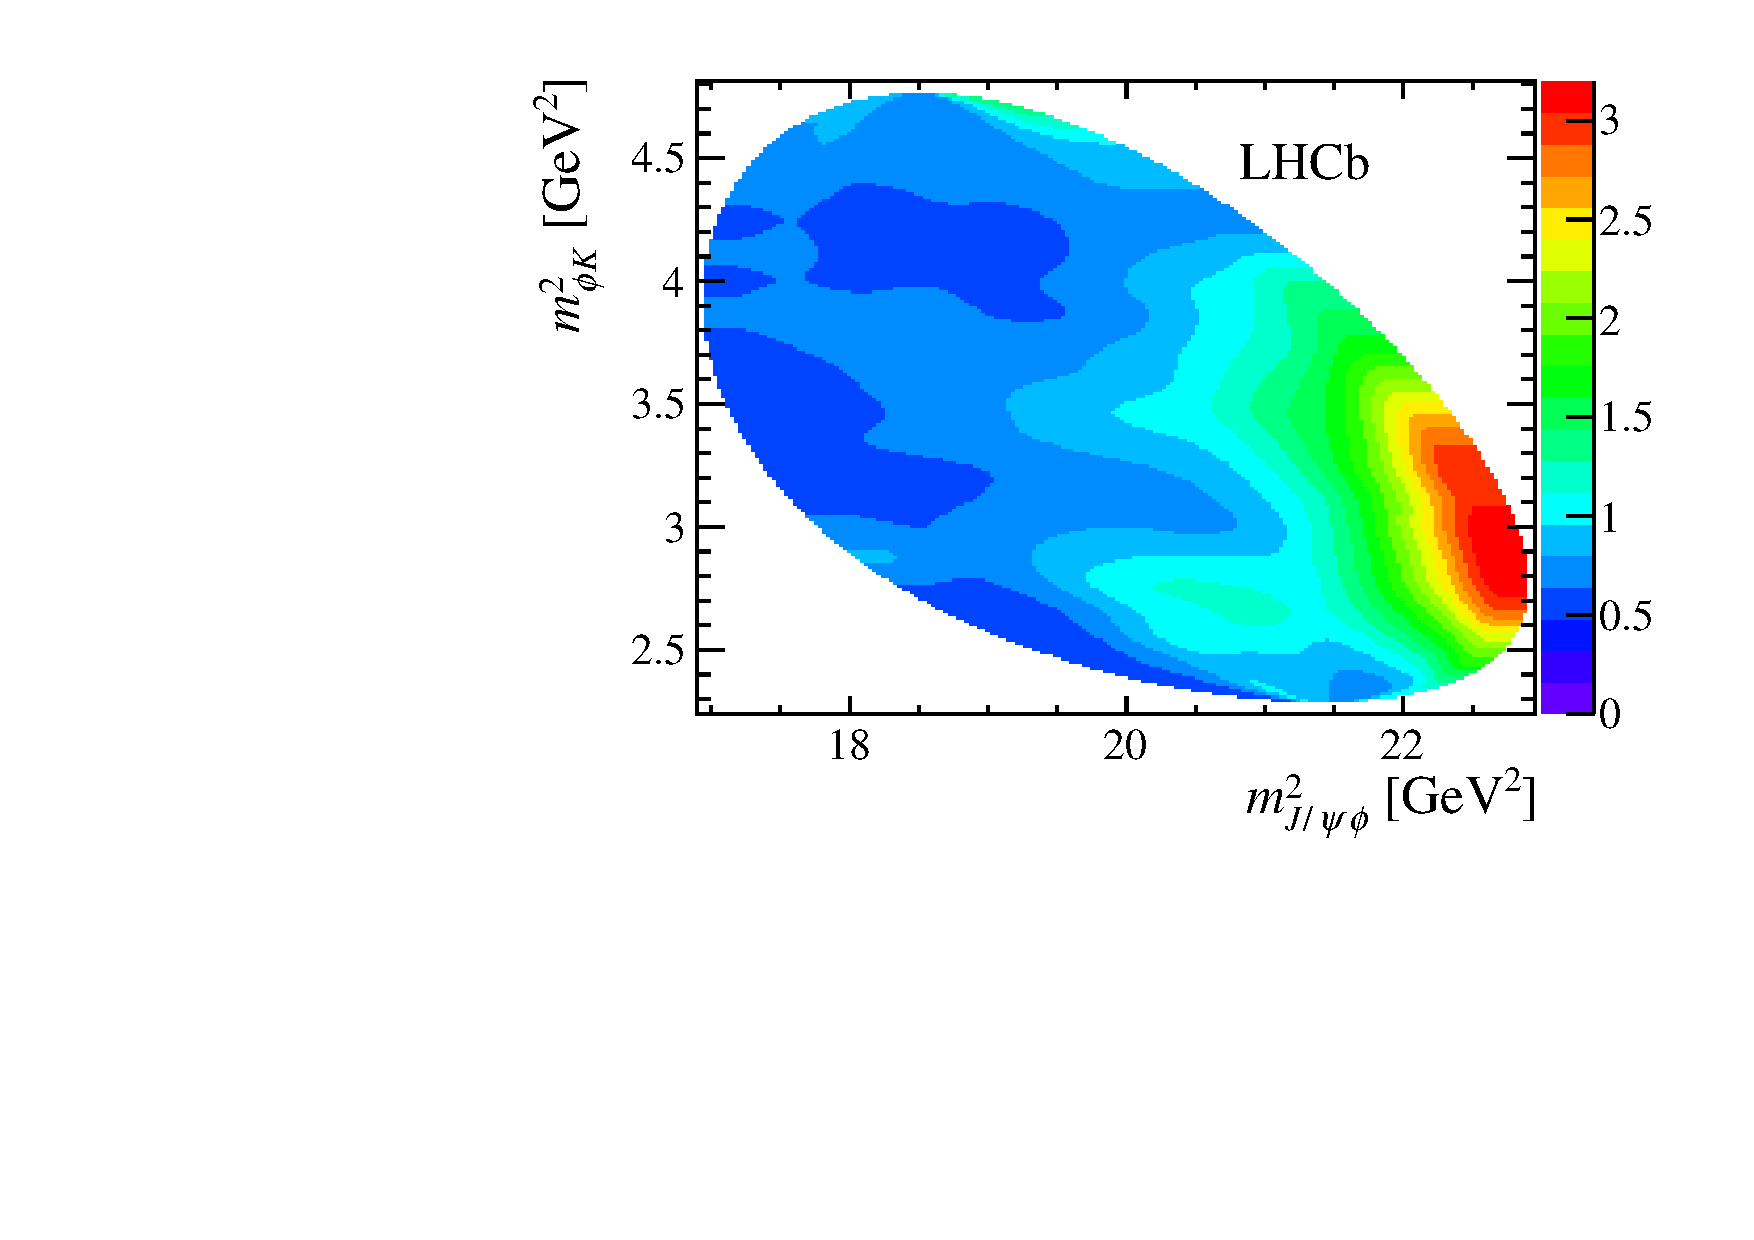
\includegraphics[width=0.8\textwidth]{Figures/05_Likelihood/bkgm1m2}
  \end{center}
  \vskip-0.3cm\caption{
     Parameterized background representation in the Dalitz plane $({\mjpsiphi^2},{\mphik^2})$.
     Function values corresponding to the color encoding are given on the right.
     The normalization arbitrarily corresponds to unity when averaged over the phase space.
  \label{fig:bkgdaleffs}
  }
\end{figure}

\begin{figure}[tbhp]
  \begin{center}
    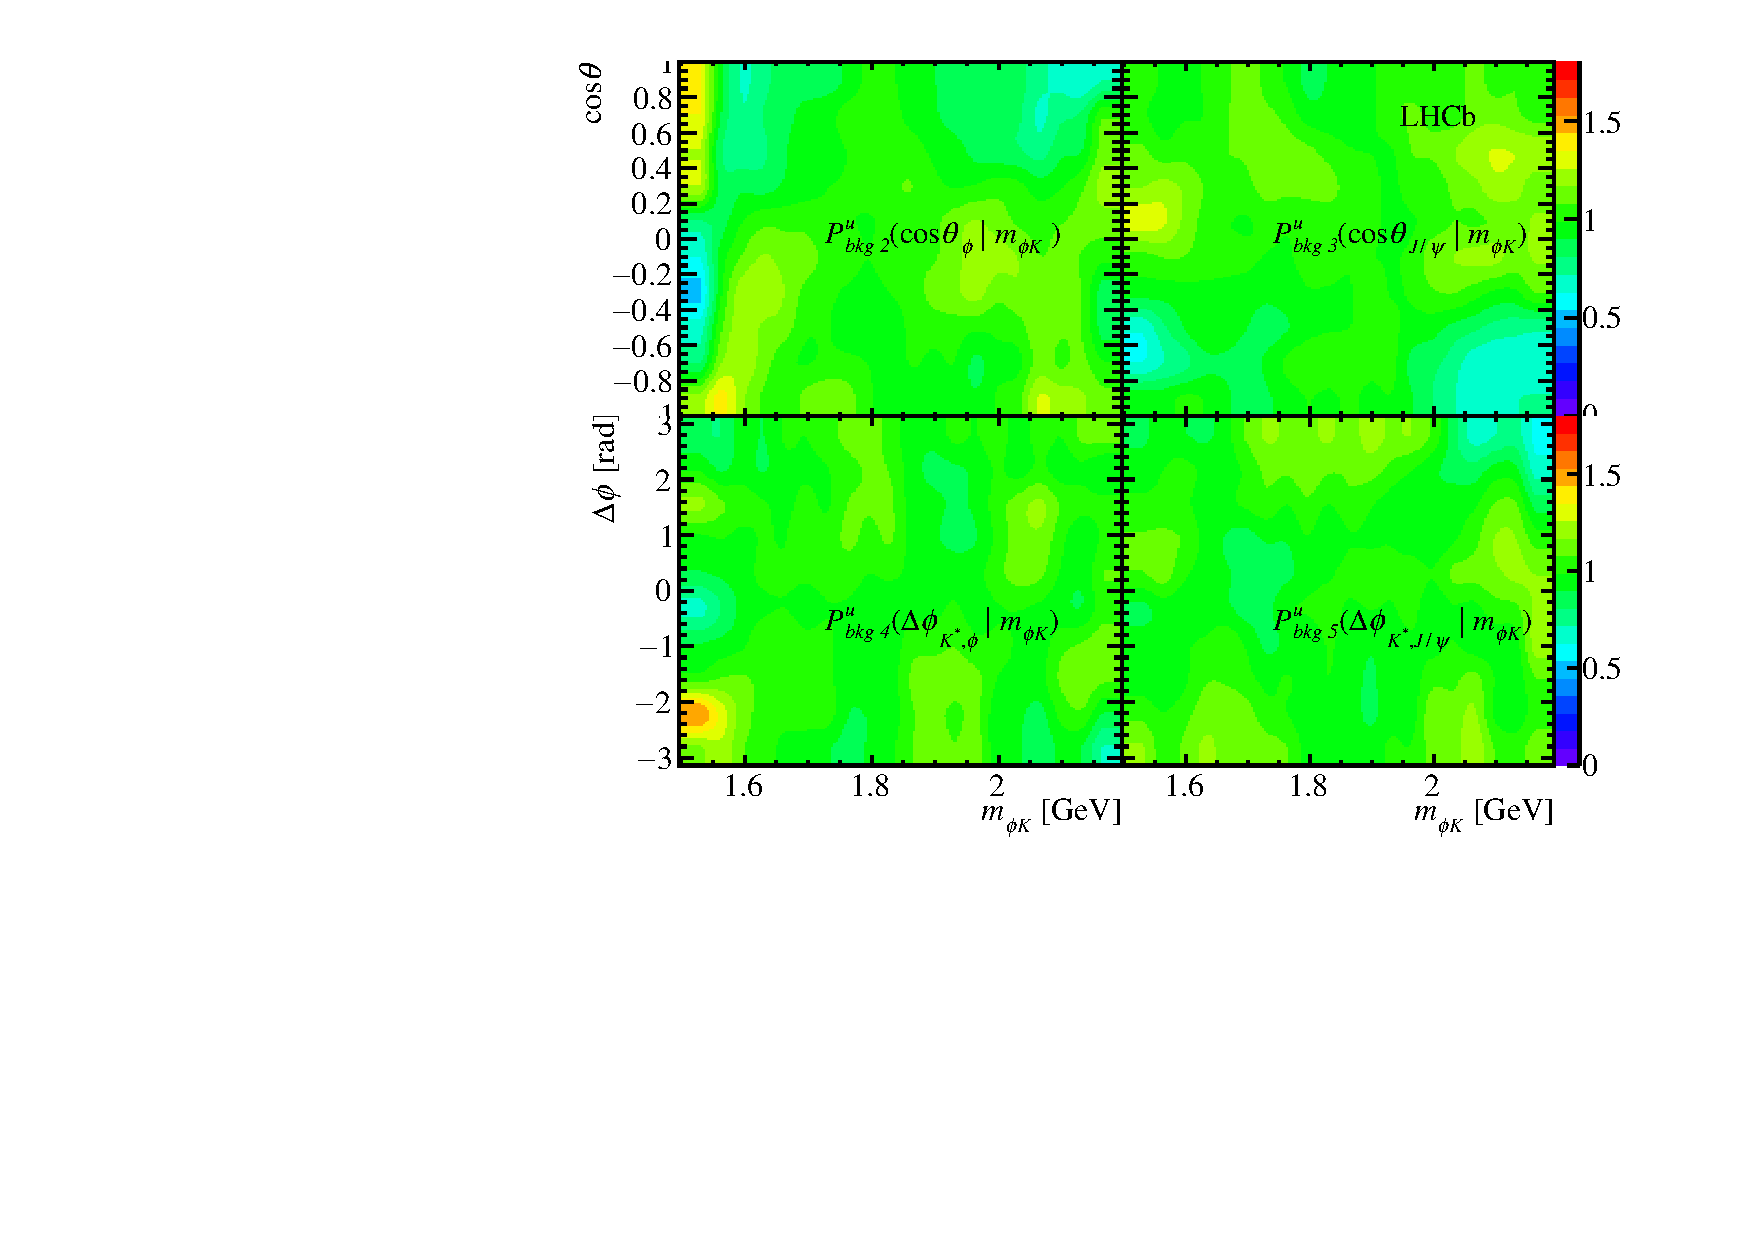
\includegraphics[width=0.8\textwidth]{Figures/05_Likelihood/bkgAngles} 
  \end{center}
  \vskip-0.3cm\caption{
     Parameterized background functions: $P^u_{\rm bkg\,2}(\cosphi|m_{\phiz\kaon})$,
     $P^u_{\rm bkg\,3}(\cospsi|m_{\phiz\kaon})$, $P^u_{\rm bkg\,4}(\phiksphi|m_{\phiz\kaon})$,
     $P^u_{\rm bkg\,5}(\phikspsi|m_{\phiz\kaon})$.
     Function values corresponding to the color encoding are given on the right.
     By construction each function integrates to unity at each $m_{\phi K}$ value.  
  \label{fig:bkgeffs2345}
  }
\end{figure}

The fit fraction (\FiFr) of any component $R$ is defined as,
\begin{equation}
\FiFr = \frac{
\int \left|\Mat^R(m_{\phi K},\Omega)\right|^2 \Phi(m_{\phi K})\,dm_{\phi K}d\Omega
}{
\int \left|\Mat(m_{\phi K},\Omega)\right|^2 \Phi(m_{\phi K})\,dm_{\phi K}d\Omega
},
\label{eq:ff}
\end{equation}
where in $\Mat^R$ 
all terms except those associated with the $R$ amplitude are set to zero. 



